

    \item Airplanes A and B are flying with constant velocity in the same vertical plane at angles \(30^\circ\) and \(60^\circ\) with respect to the horizontal respectively as shown in figure. The speed of A is \(100\sqrt{3}\) m s\(^{-1}\). At time \(t = 0\) s, an observer in A finds B at a distance of 500 m. This observer sees B moving with a constant velocity perpendicular to the line of motion of A. If at \(t = t_0\), A just escapes being hit by B, \(t_0\) in seconds is \underline{\hspace{2.5 cm}}.

    \begin{center}
        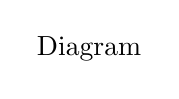
\begin{tikzpicture}
            \node {Diagram};
        \end{tikzpicture}
    \end{center}

